% XCircuit output "vsense.tex" for LaTeX input from vsense.eps
\def\putbox#1#2#3#4{\makebox[0in][l]{\makebox[#1][l]{}\raisebox{\baselineskip}[0in][0in]{\raisebox{#2}[0in][0in]{\scalebox{#3}{#4}}}}}
\def\rightbox#1{\makebox[0in][r]{#1}}
\def\centbox#1{\makebox[0in]{#1}}
\def\topbox#1{\raisebox{-0.60\baselineskip}[0in][0in]{#1}}
\def\midbox#1{\raisebox{-0.20\baselineskip}[0in][0in]{#1}}
   \scalebox{0.7}{
   \normalsize
   \parbox{3.61979in}{
   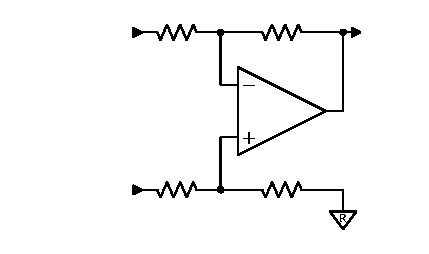
\includegraphics[scale=1.42857]{vsense}\\
   % translate x=712 y=506 scale 0.26
   \putbox{1.03in}{1.95in}{1.20}{\rightbox{\midbox{Sense$-$}}}%
   \putbox{1.03in}{0.45in}{1.20}{\rightbox{\midbox{Sense$+$}}}%
   \putbox{3.36in}{1.95in}{1.20}{\midbox{Out}}%
   } % close 'parbox'
   } % close 'scalebox'
   \vspace{-\baselineskip} % this is not necessary, but looks better
